\documentclass[polish,12pt,a4paper]{extarticle}
\usepackage[T1]{fontenc}

\usepackage[top=2.5cm,bottom=2cm,left=2cm,right=2cm]{geometry}
\usepackage{xcolor}

\usepackage{placeins}  % in the preamble
\usepackage{babel}
\usepackage{titling}
\usepackage{lastpage}
\usepackage{amsmath}
\usepackage{amssymb}
\usepackage{stmaryrd}
\usepackage{fancyhdr}
\usepackage[bookmarks=false]{hyperref}
\usepackage{algorithm2e}
\usepackage{mathtools}
\usepackage{xcolor}
%\usepackage{overarrows}
\pagestyle{fancy}


\usepackage{graphicx}
\usepackage{caption}
\usepackage{subcaption}
\usepackage[margin=1in]{geometry}

\usepackage{tikz}
\usetikzlibrary{angles,quotes}

\title{Miniprojekt 4}
\author{Jakub Wieliczko}

\fancyhead[l]{MPUM}
\fancyhead[c]{\textbf{\thetitle}}
\fancyhead[r]{\theauthor}
\fancyfoot[c]{\begin{NoHyper}\thepage/\pageref{LastPage}\end{NoHyper}}

\newcommand{\inident}{\hspace{1.25em}}

% Algo stuff
\newcommand\mycommfont[1]{\ttfamily\textcolor{gray}{#1}}
\SetCommentSty{mycommfont}
\newcommand\Field[2]{\textbf{Field} $#1$: \texttt{#2}\;}
\newcommand\Method[3]{
	\SetKwFunction{Fn#1#2}{#1.#2}
	\SetKwFunction{FnLocal#1#2}{#2}
	\MethodImpl{\textnormal{\texttt{#2}(#3)}}
}
\newcommand\Struct[1]{
	\SetKwFunction{St#1}{#1}
	\StructImpl{\textnormal{\texttt{#1}}}
}

\newcommand\initalgorithm{
	\SetAlgoLined
	\DontPrintSemicolon
	\SetKwProg{Fn}{function}{:}{end}
	\SetKwProg{StructImpl}{struct}{:}{end}
	\SetKwProg{MethodImpl}{method}{:}{end}
}

% Math Stuff
\newcommand\Nat{\mathbb{N}}
\newcommand\Primes{\mathbb{P}}
\newcommand\eqqm[0]{\stackrel{?}{=}}
\renewcommand\lor{\,\vee\,}
\renewcommand\land{\,\wedge\,}
\newcommand\lxor[0]{\,\veebar\,}
\newcommand\union[0]{\cup}
\newcommand\isect[0]{\cap}
\newcommand\Union[0]{\bigcup}
\newcommand\Isect[0]{\bigcap}
\newcommand\nil[0]{\emptyset}
\renewcommand\geq{\geqslant}
\renewcommand\leq{\leqslant}
\newcommand\eqs[1]{\stackrel{#1}{=}}
\newcommand\impliesqm[0]{\stackrel{?}{\implies}}
\newcommand\QED[0]{\hfill$\blacksquare$}

\newcommand\set[1]{\left\{#1\right\}}
\newcommand\card[1]{\left|#1\right|}
\newcommand\cset[1]{\card{\set{#1}}}
\DeclarePairedDelimiter{\floor}{\lfloor}{\rfloor}
\DeclarePairedDelimiter{\ceil}{\lceil}{\rceil}

\newcommand{\stirC}[2]{\genfrac{[}{]}{0pt}{}{#1}{#2}}
\newcommand{\stirP}[2]{\genfrac{\{}{\}}{0pt}{}{#1}{#2}}


%\NewOverArrowCommand{image}{}
%\NewOverArrowCommand{coimage}{
%	end=\leftarrow
%}

\newcommand\stdarr[0]{\rightarrow}
\newcommand\injarr[0]{\hookrightarrow}
\newcommand\surarr[0]{\rightarrow\mathrel{\mspace{-15mu}}\rightarrow}
\newcommand\bijarr[0]{\hookrightarrow\mathrel{\mspace{-15mu}\rightarrow}}

\begin{document}
\begin{abstract}
W poniższym dokumencie opisuję moją pracę w związku z 4 miniprojektem z MPUM, dotyczącym algorytmów klasteryzacji
\end{abstract}
\section*{Wprowadzenie}
Na potrzeby tego projektu porównuję działanie algorytmów \texttt{klasteryzacji hierarchicznej} \texttt{algorytmu k-średnich} i \texttt{klasteryzacji spektralnej}. W pierwszej części raportu zajmę się wyznaczaniem liczby klastrów dla zbiorów  \texttt{dane\_18D.txt} i \texttt{dane\_2D\_n.txt}. Następnie dla każdego z algorytmów porównam jego działanie na zbiorach \texttt{rp.data}, \texttt{dane\_2D\_n.txt} dla $k$ będącego podaną liczbą klas, zaś dla pliku \texttt{dane\_18D.txt} wyznaczę wartość $k$ w oparciu o później opisane metody. Na początku przyjrzyjmy się podanym zbiorom 2D.
\section{Dane 2D}
Do miniprojektu zostały dołączone dane 2D. Żeby wiedzieć z czym pracujemy poniżej zamieszczam ich wizualizację, wraz z opisem liczby klas.

\begin{figure}[h!]
    \centering
    \begin{subfigure}[b]{0.30\textwidth}
        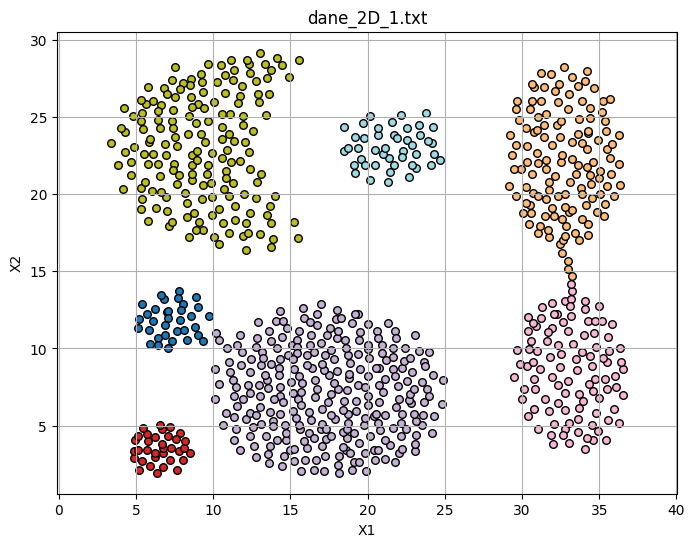
\includegraphics[width=\linewidth]{img/data/dane1.png}
        \captionsetup{labelformat=empty}
        \caption{Zestaw 1: 7 Klas}
    \end{subfigure}
    \hfill
    \begin{subfigure}[b]{0.30\textwidth}
        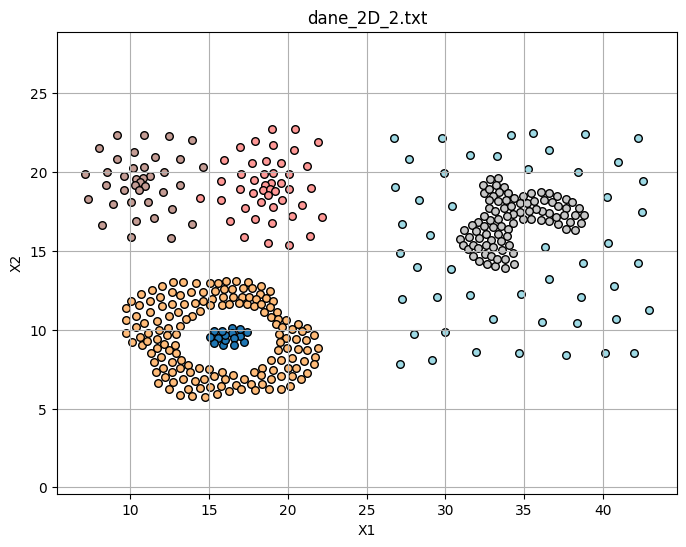
\includegraphics[width=\linewidth]{img/data/dane2.png}
        \captionsetup{labelformat=empty}
        \caption{Zestaw 2: 6 Klas}
    \end{subfigure}
    \hfill
    \begin{subfigure}[b]{0.30\textwidth}
        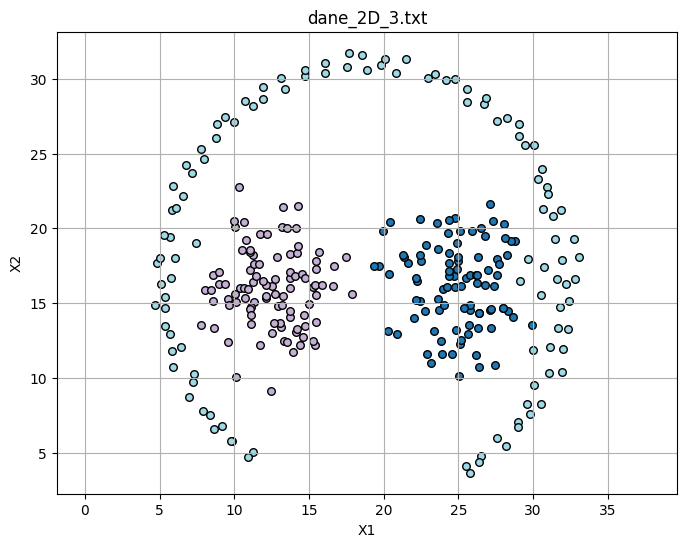
\includegraphics[width=\linewidth]{img/data/dane3.png}
        \captionsetup{labelformat=empty}
        \caption{Zestaw 3: 3 Klas}
    \end{subfigure}
    \hfill
    \begin{subfigure}[b]{0.30\textwidth}
        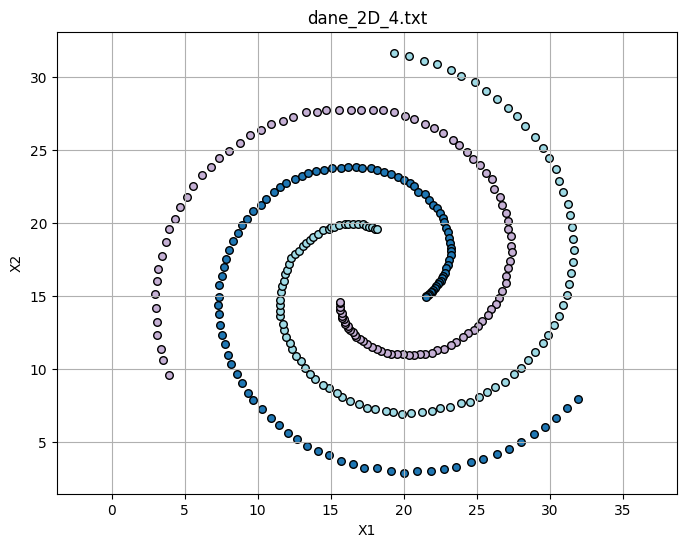
\includegraphics[width=\linewidth]{img/data/dane4.png}
        \captionsetup{labelformat=empty}
        \caption{Zestaw 4: 3 Klas}
    \end{subfigure}
    \hfill
    \begin{subfigure}[b]{0.30\textwidth}
        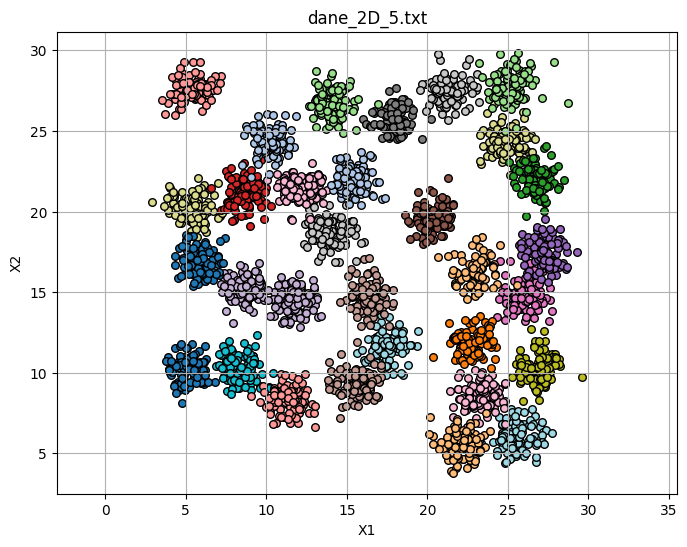
\includegraphics[width=\linewidth]{img/data/dane5.png}
        \captionsetup{labelformat=empty}
        \caption{Zestaw 5: 31 Klas}
    \end{subfigure}
    \hfill
    \begin{subfigure}[b]{0.30\textwidth}
        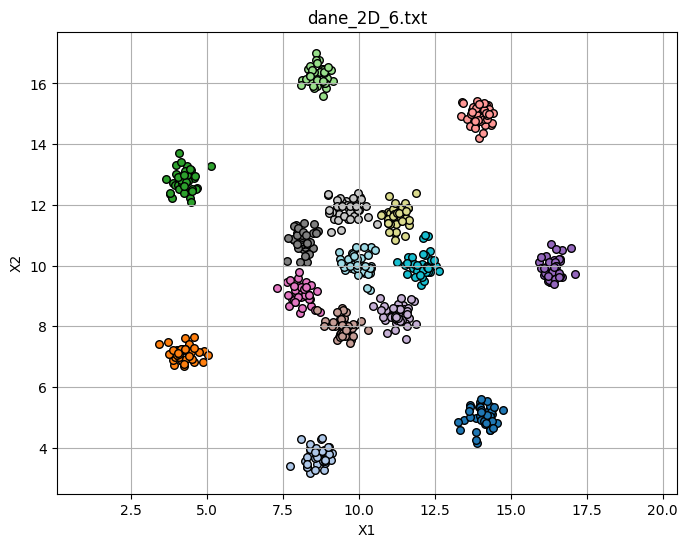
\includegraphics[width=\linewidth]{img/data/dane6.png}
        \captionsetup{labelformat=empty}
        \caption{Zestaw 6: 15 Klas}
    \end{subfigure}
    \hfill
    \vspace{}
    \begin{subfigure}[b]{0.30\textwidth}
        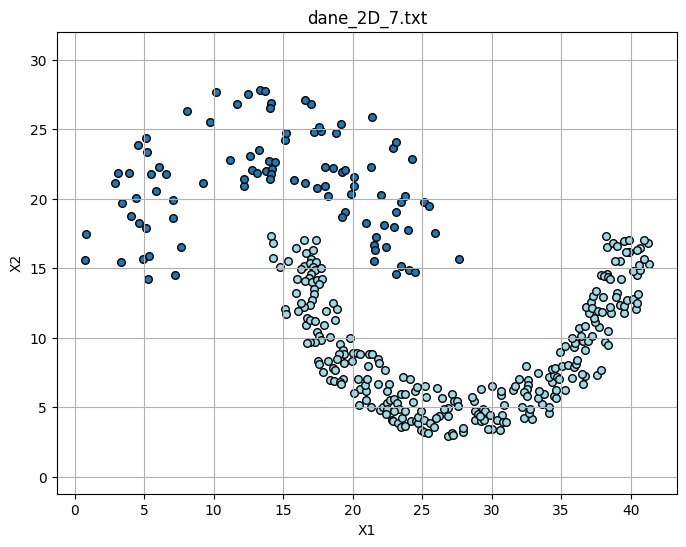
\includegraphics[width=\linewidth]{img/data/dane7.png}
        \captionsetup{labelformat=empty}
        \caption{Zestaw 7: 2 Klasy}
    \end{subfigure}
    \begin{subfigure}[b]{0.30\textwidth}
        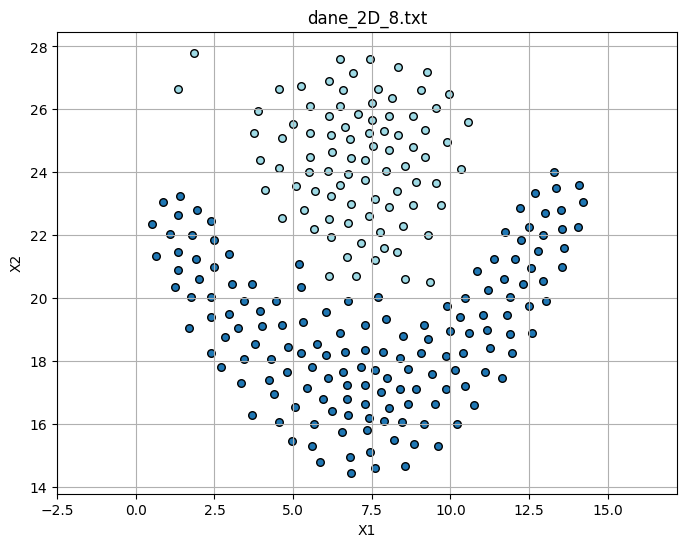
\includegraphics[width=\linewidth]{img/data/dane8.png}
        \captionsetup{labelformat=empty}
        \caption{Zestaw 8: 2 Klasy}
    \end{subfigure}
    \label{fig:data_grid}
\end{figure} \smallskip \\
\noindent Przyglądając się danym widzimy, że wiele z tych klasyfikacji nie daje kształtów kulistych, w związku z czym zakładam że algorytmy takie jak \texttt{k-średnich}, czy niektóre metody łączenia w \texttt{grupowaniu hierarchicznym} mogą dawać odmienne od zadanych wyniki. Zanim jednak do tego przejdziemy, spróbujmy wyznaczyć liczbę klastrów dla naszych zbiorów danych.

\section*{Wyznaczanie liczby klastrów}
Spróbujmy do tego skorzystać z metody łokciowej. Poniżej przedstawiam wykresy kolejnych wykresów błędu względem liczby klas w metodzie \texttt{k-średnich}


\begin{figure}[h!]
    \centering
    \begin{subfigure}[b]{0.30\textwidth}
        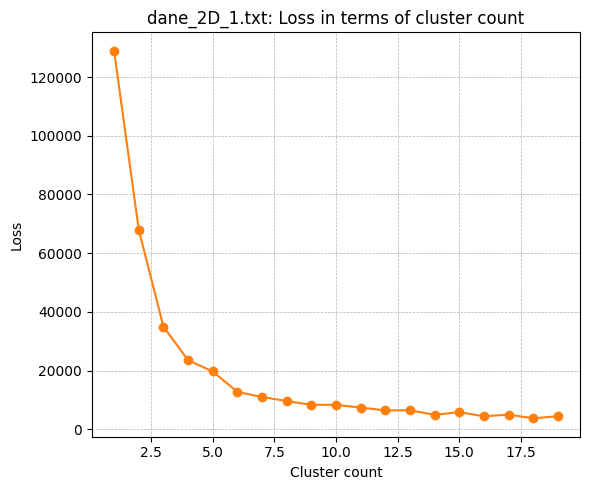
\includegraphics[width=\linewidth]{img/elbow/data1.png}
        \captionsetup{labelformat=empty}
    \end{subfigure}
    \hfill
    \begin{subfigure}[b]{0.30\textwidth}
        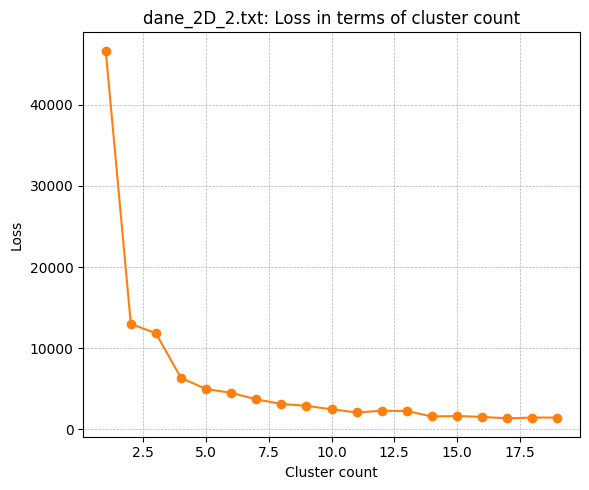
\includegraphics[width=\linewidth]{img/elbow/data2.png}
        \captionsetup{labelformat=empty}
    \end{subfigure}
    \hfill
    \begin{subfigure}[b]{0.30\textwidth}
        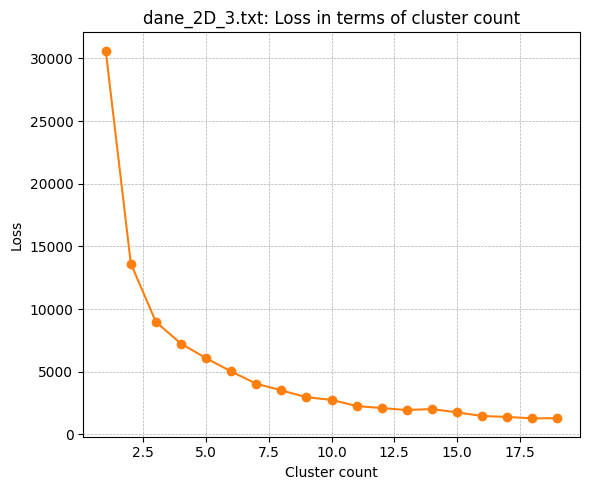
\includegraphics[width=\linewidth]{img/elbow/data3.png}
        \captionsetup{labelformat=empty}
    \end{subfigure}
    \hfill
    \begin{subfigure}[b]{0.30\textwidth}
        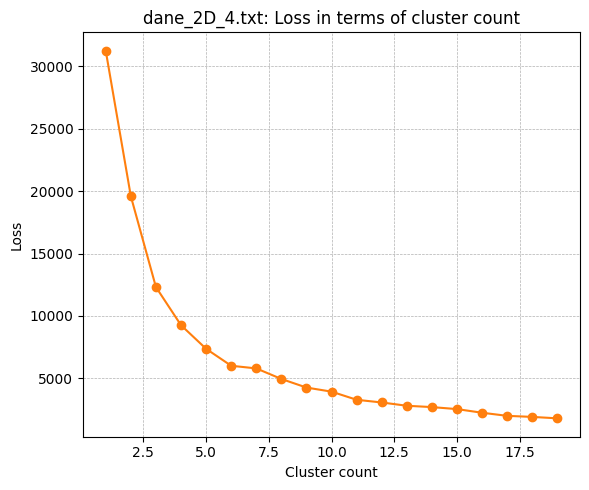
\includegraphics[width=\linewidth]{img/elbow/data4.png}
        \captionsetup{labelformat=empty}
    \end{subfigure}
    \hfill
    \begin{subfigure}[b]{0.30\textwidth}
        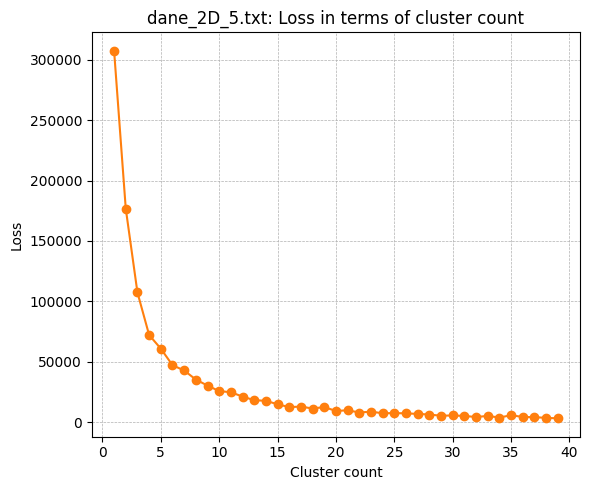
\includegraphics[width=\linewidth]{img/elbow/data5.png}
        \captionsetup{labelformat=empty}
    \end{subfigure}
    \hfill
    \begin{subfigure}[b]{0.30\textwidth}
        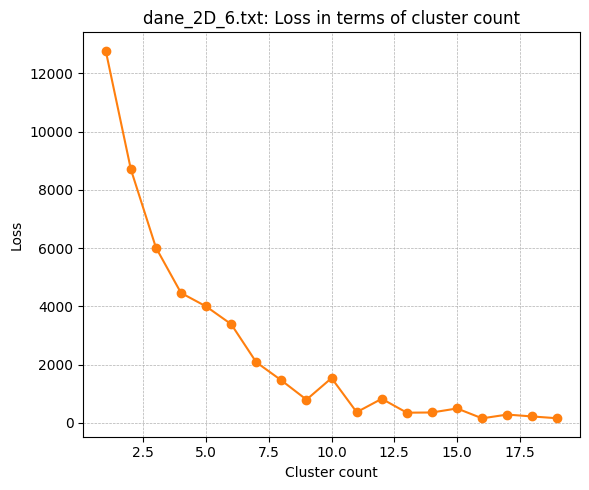
\includegraphics[width=\linewidth]{img/elbow/data6.png}
        \captionsetup{labelformat=empty}
    \end{subfigure}
    \hfill
    \vspace{}
    \begin{subfigure}[b]{0.30\textwidth}
        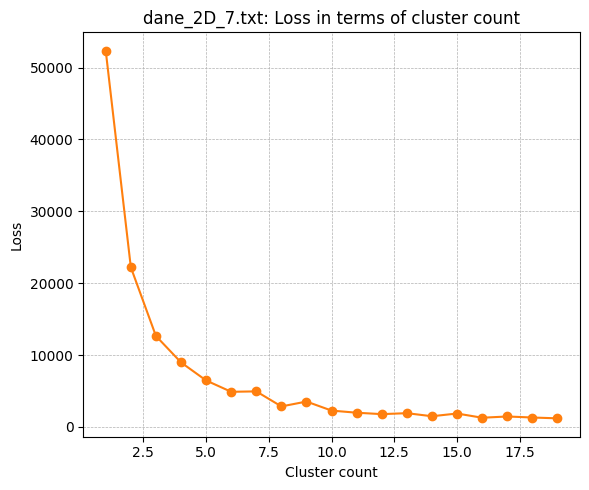
\includegraphics[width=\linewidth]{img/elbow/data7.png}
        \captionsetup{labelformat=empty}
    \end{subfigure}
    \begin{subfigure}[b]{0.30\textwidth}
        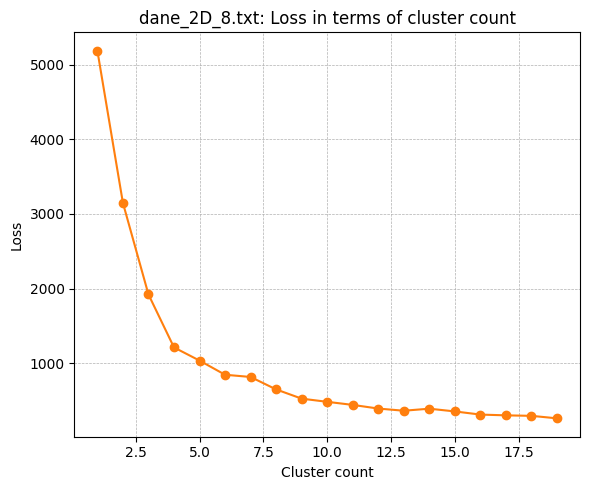
\includegraphics[width=\linewidth]{img/elbow/data8.png}
        \captionsetup{labelformat=empty}
    \end{subfigure}
    \label{fig:data_grid}
\end{figure} \\
\noindent Widzimy, że pierwszy i drugi wykres się wypłaszcza po $k = 6$, zaś szósty przy $k = 15$, a przy siódmym i ósmym wykresie najwiekszy spadek jest przy $k = 2$. Jednak korzystając z tej metody ciężko jednoznacznie wyznaczyć liczbę klastrów. W późniejszej części raportu przeanalizujemy resztę zbiorów korzystając z innej metody.


\section*{Miara dokładności}
Przed dalszą częścią materiału zaznączę tylko, że dokładność mierzę w ten sposób że spośród wszystkich par punktów $(X, Y)$ ze zbioru w którym znamy klastry patrzę czy $X, Y$ są klasyfikowane przez model jako należące do jednej klasy wtedy i tylko wtedy gdy w danych testowych też należą do jednej klasy. Wtedy dokładnością jest średnia wartość tego po wszystkich parach $(X, Y)$.

\section*{Algorytm k-średnich}

Na początek przeanalizujmy wyniki które zwrócił algorytm \texttt{k-średnich}.
Dla danych 2D uruchomiłem algorytm na tylu klasach, ile zostało wyszczególnionych wśród danych wejściowych. Poniżej znajdują się wyniki podziału tych danych na klasy. Spośród wszystkich metryk które testowałem najciekawsze wyniki dała \texttt{metryka Euklidesowa}, więc jej wynikami się zajmijmy

\begin{figure}[h!]
    \centering

    \begin{subfigure}[b]{0.30\textwidth}
        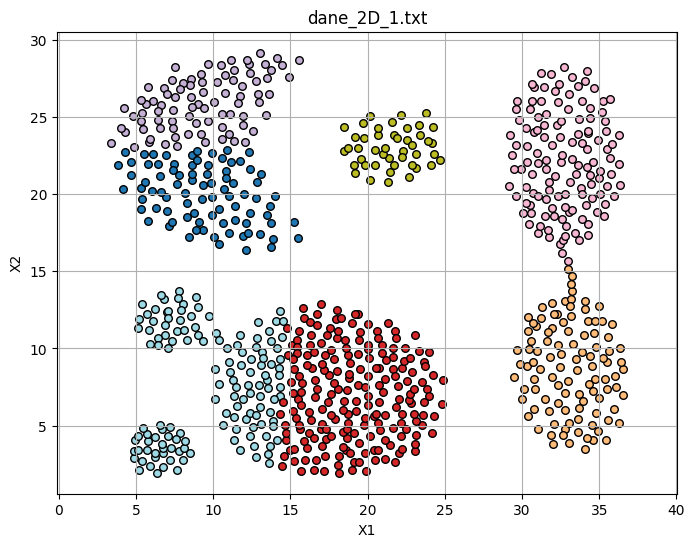
\includegraphics[width=\linewidth]{img/kmeans2D/data1.png}
        \captionsetup{labelformat=empty}
        \caption{Zestaw 1: 7 Klas}
    \end{subfigure}
    \hfill
    \begin{subfigure}[b]{0.30\textwidth}
        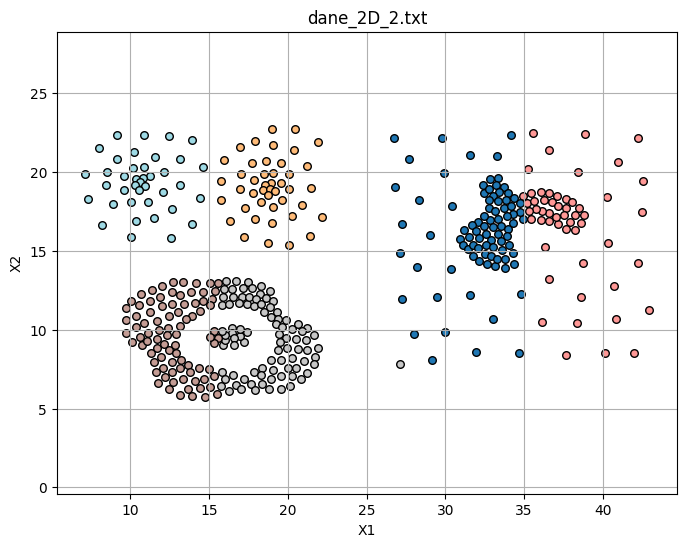
\includegraphics[width=\linewidth]{img/kmeans2D/data2.png}
        \captionsetup{labelformat=empty}
        \caption{Zestaw 2: 6 Klas}
    \end{subfigure}
    \hfill
    \begin{subfigure}[b]{0.30\textwidth}
        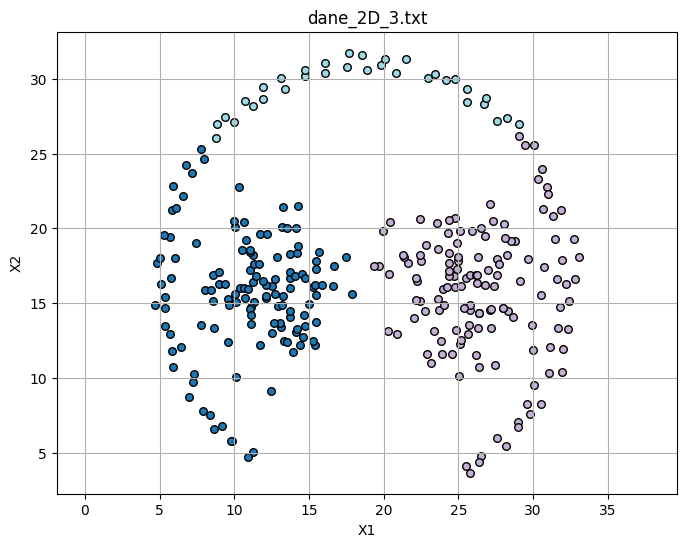
\includegraphics[width=\linewidth]{img/kmeans2D/data3.png}
        \captionsetup{labelformat=empty}
        \caption{Zestaw 3: 3 Klas}
    \end{subfigure}
    \hfill
    \begin{subfigure}[b]{0.30\textwidth}
        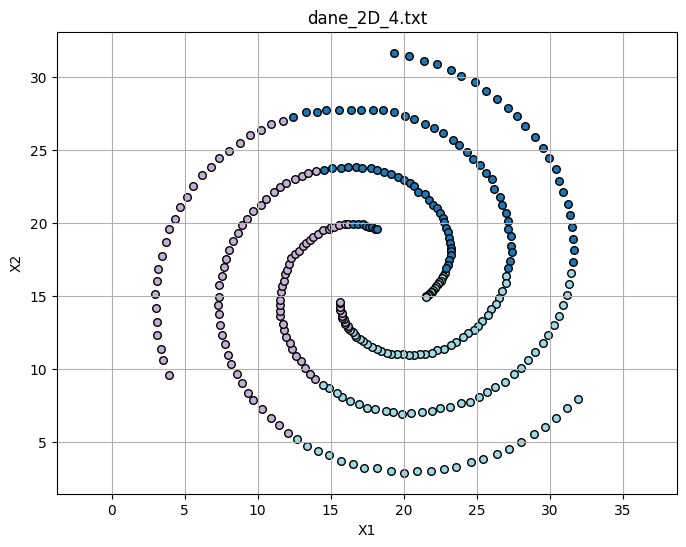
\includegraphics[width=\linewidth]{img/kmeans2D/data4.png}
        \captionsetup{labelformat=empty}
        \caption{Zestaw 4: 3 Klas}
    \end{subfigure}
    \hfill
    \begin{subfigure}[b]{0.30\textwidth}
        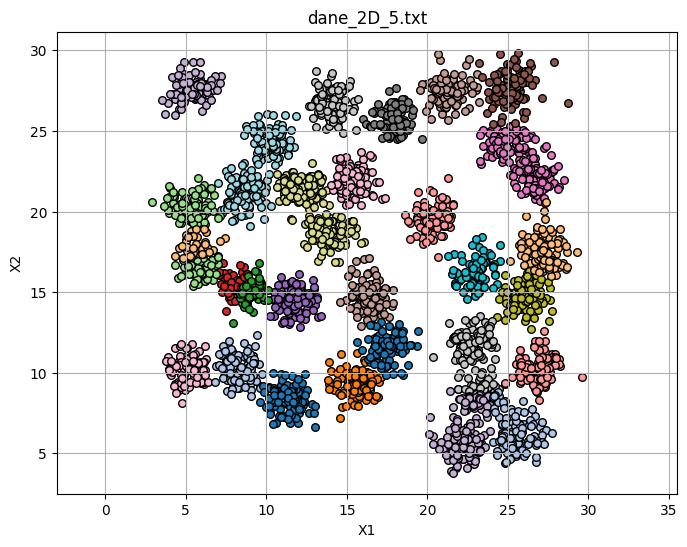
\includegraphics[width=\linewidth]{img/kmeans2D/data5.png}
        \captionsetup{labelformat=empty}
        \caption{Zestaw 5: 31 Klas}
    \end{subfigure}
    \hfill
    \begin{subfigure}[b]{0.30\textwidth}
        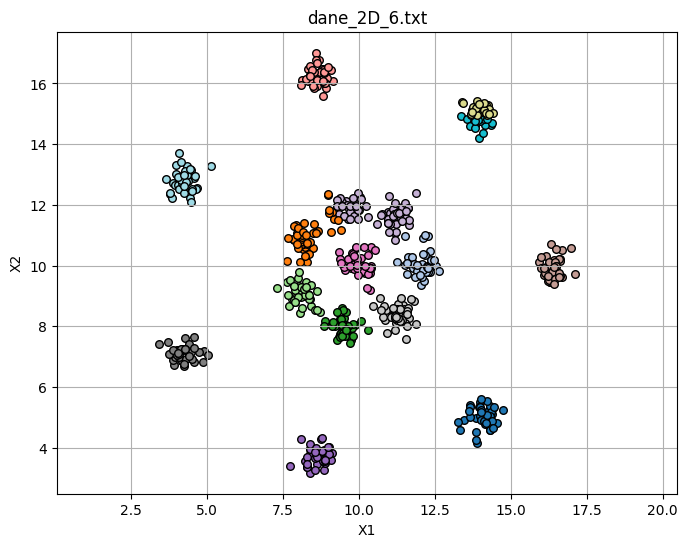
\includegraphics[width=\linewidth]{img/kmeans2D/data6.png}
        \captionsetup{labelformat=empty}
        \caption{Zestaw 6: 15 Klas}
    \end{subfigure}
    \hfill
    \vspace{}
    \begin{subfigure}[b]{0.30\textwidth}
        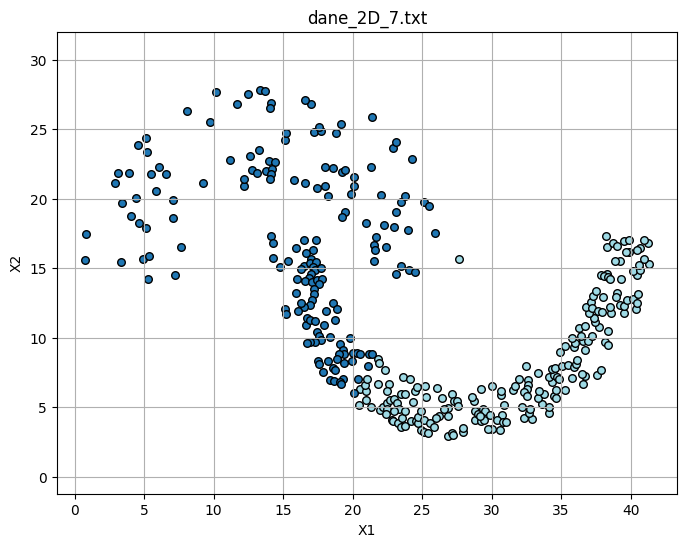
\includegraphics[width=\linewidth]{img/kmeans2D/data7.png}
        \captionsetup{labelformat=empty}
        \caption{Zestaw 7: 2 Klasy}
    \end{subfigure}
    \begin{subfigure}[b]{0.30\textwidth}
        \includegraphics[width=\linewidth]{img/kmeans2D/data8.png}
        \captionsetup{labelformat=empty}
        \caption{Zestaw 8: 2 Klasy}
    \end{subfigure}
    \label{fig:data_grid}
\end{figure}

\noindent Wnioski są dosyć spodziewane, algorytm bardzo ładnie poradził sobie  w zestawach 5 i 6, gdzie rozważane dane były kuliste. Również nienagannie zaklasyfikował niektóre klasy spośród zestawu 1 i 2, oraz przyzwoicie poradził sobie z zestawami 7 i 8. Największy problem miał on w zestawach 3 i 4, gdzie szukane klasy nie są skupione wokół punktów, tylko dane w jednej klasie zależą od siebie w inny sposób. Spójrzmy na wyniki naszego modelu na poszczególnych zestawach danych.\\

\begin{table}[h!]
\centering
\begin{tabular}{|l|c|}
\hline
\textbf{Zestaw} & \textbf{Dokładność} \\
\hline
Dane nr 1 & 0.927 \\
Dane nr 2 & 0.906 \\
Dane nr 3 & 0.749 \\
Dane nr 4 & 0.554 \\
Dane nr 5 & 0.979 \\
Dane nr 6 & 0.974 \\
Dane nr 7 & 0.662 \\
Dane nr 8 & 0.744 \\
\hline
\end{tabular}
\caption{Dokładności algorytmu k-średnich}
\label{tab:metrics}
\end{table}

\section*{Algorytm grupowania hierarchicznego}
Na początek zdecydowałem się sprawdzić, jak poradzi sobie łączenie centroidalne. Poniżej przedstawiam wyniki zarówno w formie graficznej, jak i tabelki dokładności:

\begin{figure}[h!]
    \centering

    \begin{subfigure}[b]{0.30\textwidth}
        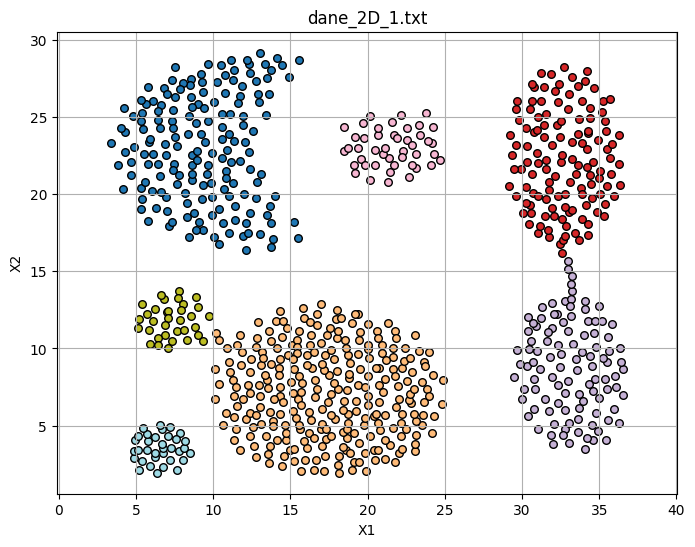
\includegraphics[width=\linewidth]{img/hierarchical/centroid/data1.png}
        \captionsetup{labelformat=empty}
        \caption{Zestaw 1: 7 Klas}
    \end{subfigure}
    \hfill
    \begin{subfigure}[b]{0.30\textwidth}
        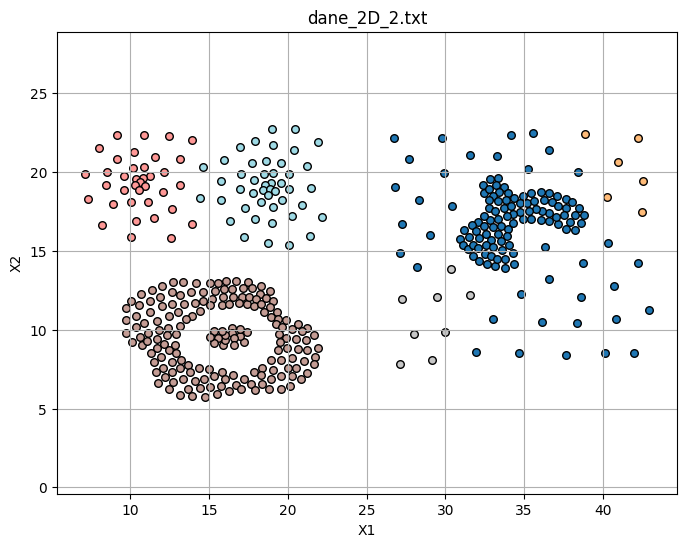
\includegraphics[width=\linewidth]{img/hierarchical/centroid/data2.png}
        \captionsetup{labelformat=empty}
        \caption{Zestaw 2: 6 Klas}
    \end{subfigure}
    \hfill
    \begin{subfigure}[b]{0.30\textwidth}
        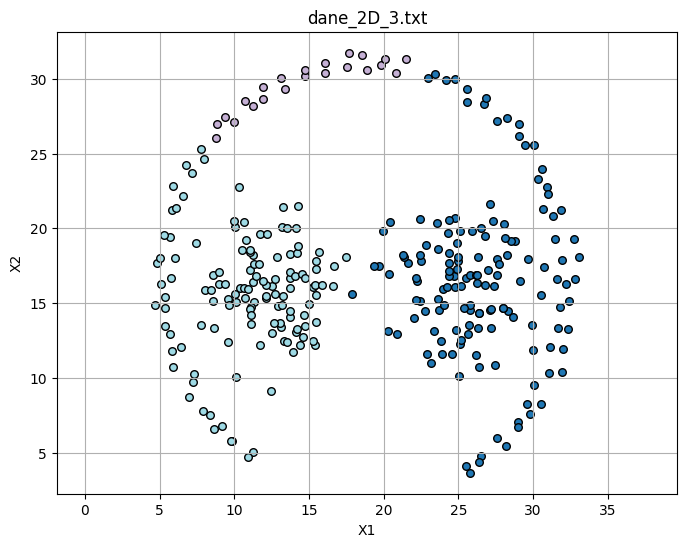
\includegraphics[width=\linewidth]{img/hierarchical/centroid/data3.png}
        \captionsetup{labelformat=empty}
        \caption{Zestaw 3: 3 Klas}
    \end{subfigure}
    \hfill
    \begin{subfigure}[b]{0.30\textwidth}
        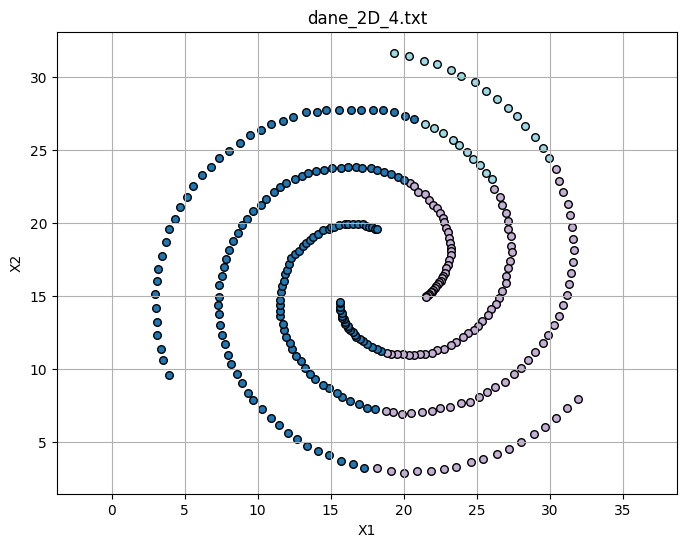
\includegraphics[width=\linewidth]{img/hierarchical/centroid/data4.png}
        \captionsetup{labelformat=empty}
        \caption{Zestaw 4: 3 Klas}
    \end{subfigure}
    \hfill
    \begin{subfigure}[b]{0.30\textwidth}
        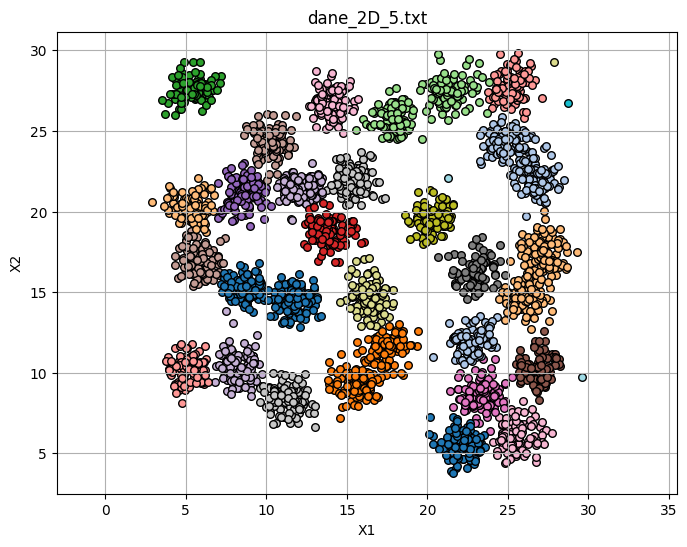
\includegraphics[width=\linewidth]{img/hierarchical/centroid/data5.png}
        \captionsetup{labelformat=empty}
        \caption{Zestaw 5: 31 Klas}
    \end{subfigure}
    \hfill
    \begin{subfigure}[b]{0.30\textwidth}
        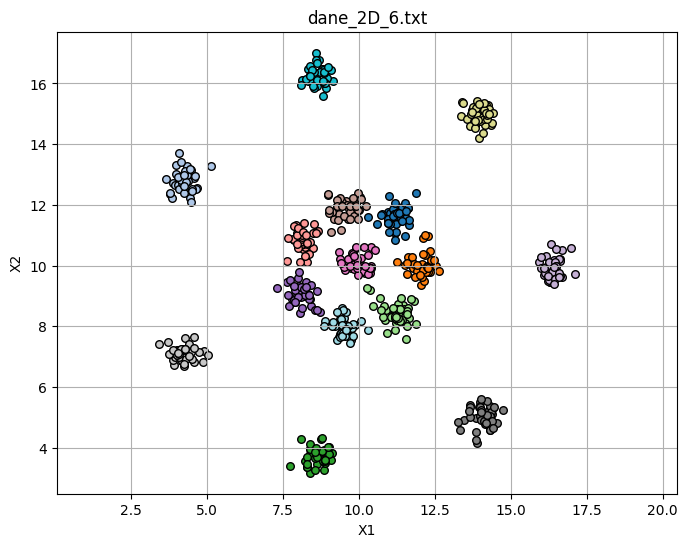
\includegraphics[width=\linewidth]{img/hierarchical/centroid/data6.png}
        \captionsetup{labelformat=empty}
        \caption{Zestaw 6: 15 Klas}
    \end{subfigure}
    \hfill
\end{figure}
\begin{figure}[h!]
    \centering
    \begin{subfigure}[b]{0.30\textwidth}
        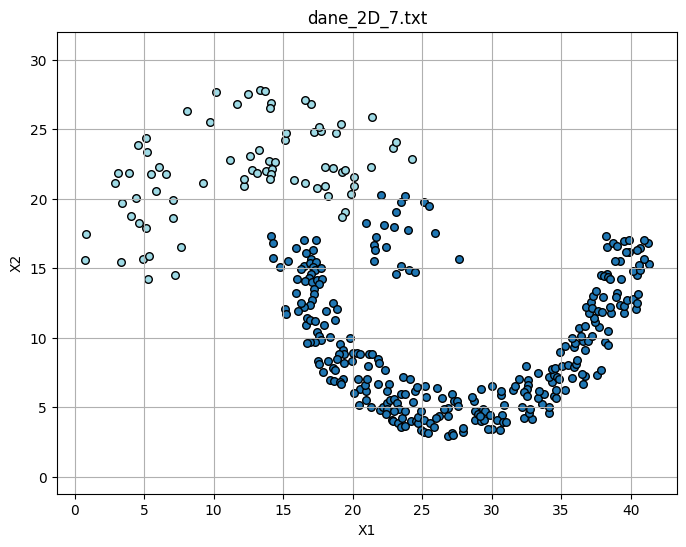
\includegraphics[width=\linewidth]{img/hierarchical/centroid/data7.png}
        \captionsetup{labelformat=empty}
        \caption{Zestaw 7: 2 Klasy}
    \end{subfigure}
    \begin{subfigure}[b]{0.30\textwidth}
        \includegraphics[width=\linewidth]{img/hierarchical/centroid/data8.png}
        \captionsetup{labelformat=empty}
        \caption{Zestaw 8: 2 Klasy}
    \end{subfigure}
    \label{fig:data_grid}
\end{figure} \FloatBarrier


\begin{table}[h!]
\centering
\begin{tabular}{|l|c|}
\hline
\textbf{Zestaw} & \textbf{Dokładność} \\
\hline
Zestaw nr 1 & 0.998 \\
Zestaw nr 2 & 0.918 \\
Zestaw nr 3 & 0.725 \\
Zestaw nr 4 & 0.526 \\
Zestaw nr 5 & 0.988 \\
Zestaw nr 6 & 0.998 \\
Zestaw nr 7 & 0.893 \\
Zestaw nr 8 & 0.541 \\
\hline
\end{tabular}
\caption{Dokładności łączenia centroidalnego}
\label{tab:metrics}
\end{table}
\noindent Porównując tą technikę do algorytmu \texttt{k-średnich}, widzimy wyższe dokładności na zbiorach 1, 5, 6 gdzie algorytm uzyskał ekstremalnie wysokie dokładności, jednak w zestawie 8 zaklasyfikował prawie wszystkie punkty do jednej klasy a tylko dwa z boku do drugiej. Mimo to nadal nie poradził sobie z klasyfikacją zestawów 3 i 4, zatem wytestujmy na nich łączenie pojedyncze.

\begin{figure}[h!]
    \centering
    \begin{subfigure}[b]{0.30\textwidth}
        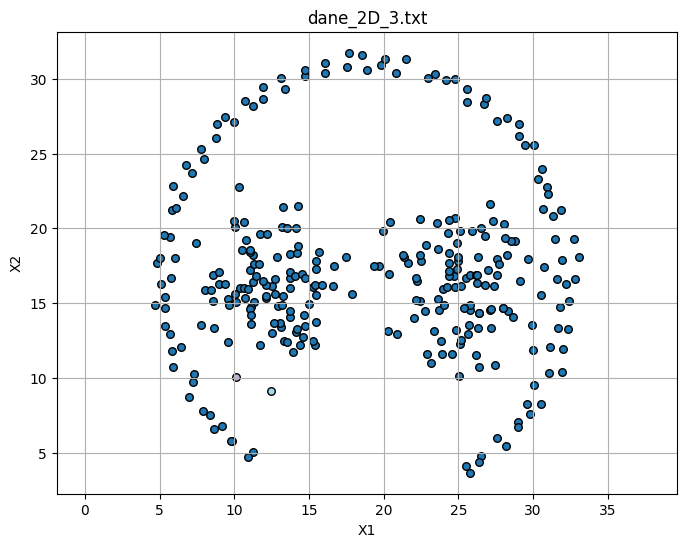
\includegraphics[width=\linewidth]{img/hierarchical/singular/data3.png}
        \captionsetup{labelformat=empty}
        \caption{Zestaw 3: Dokładność 0.337}
    \end{subfigure}
    \begin{subfigure}[b]{0.30\textwidth}
        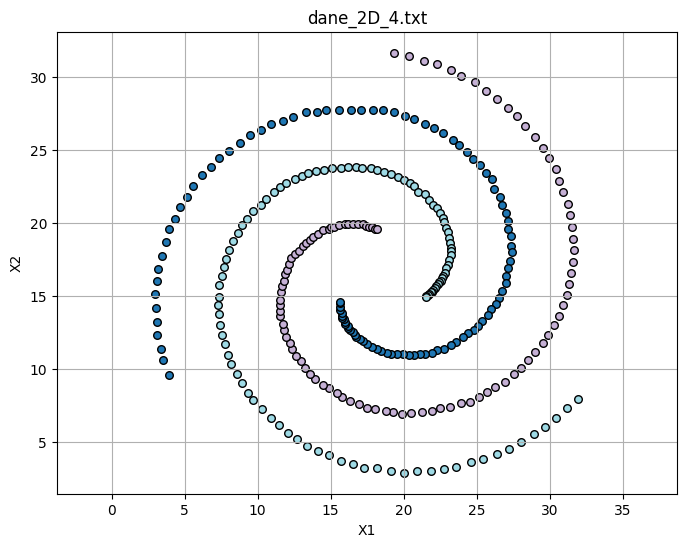
\includegraphics[width=\linewidth]{img/hierarchical/singular/data4.png}
        \captionsetup{labelformat=empty}
        \caption{Zestaw 4: Dokładność 1.000}
    \end{subfigure}
    \label{fig:data_grid}
    \caption{Wyniki łączenia pojedynczego}
\end{figure} \FloatBarrier

\noindent Widzimy, że dla zestawu 4 algorytm wszystkie punkty zaklasyfikował poprawnie, jednak nadal beznadziejnie mu poszło na zestawie 3, gdzie prawie wszystko wrzucił do jednej klasy. Testując inne metody łączenia nie uzyskałem lepszych rezultatów dla zestawu 4 niż grupowanie centroidalne.

\section*{Klasteryzacja Spektralna}
Ten algorytm zdecydowałem się napisać w oparciu o załączony do miniprojektu artykuł \texttt{On Spectral Clustering: Analysis and an algorithm}. Jedyna różnica jest taka, że po przekształceniu danych używam algorytmu \texttt{grupowania hierarchicznego} z łączeniem pojedynczym do wyznaczenia klastrów. Jeśli chodzi o parametr $\sigma$, to najlepiej sprawdzał się $\sigma = 1$. Zobaczmy jak sobie radzi z naszymi zestawami danych.


\begin{figure}[h!]
    \centering

    \begin{subfigure}[b]{0.30\textwidth}
        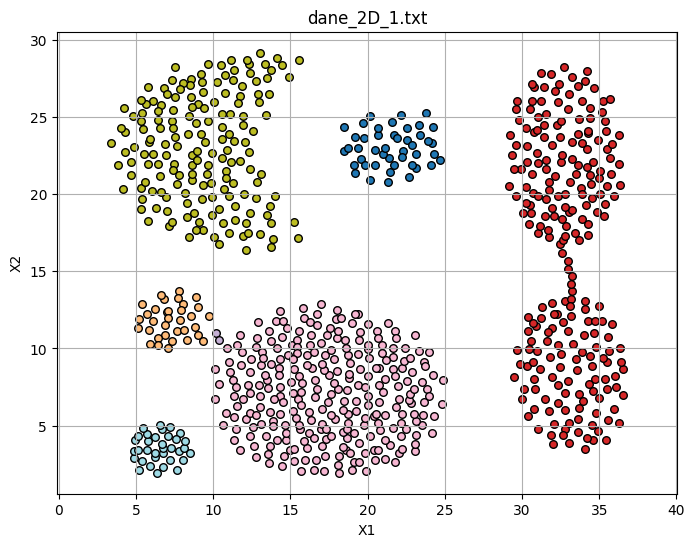
\includegraphics[width=\linewidth]{img/spectral/singular/data1.png}
        \captionsetup{labelformat=empty}
        \caption{Zestaw 1: 7 Klas}
    \end{subfigure}
    \hfill
    \begin{subfigure}[b]{0.30\textwidth}
        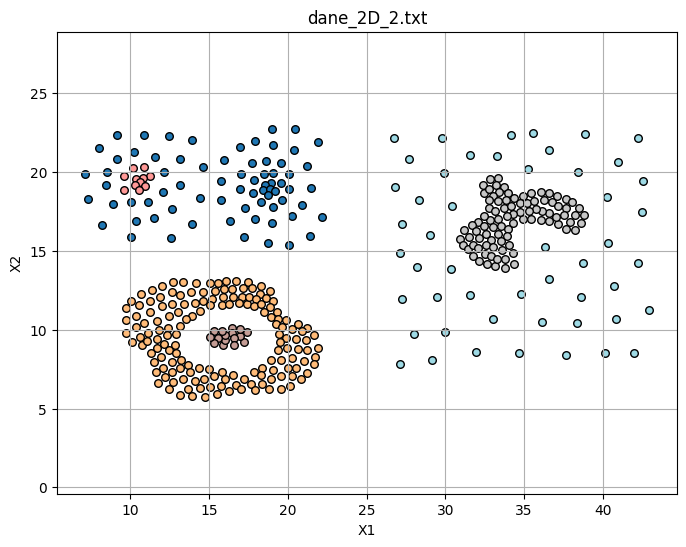
\includegraphics[width=\linewidth]{img/spectral/singular/data2.png}
        \captionsetup{labelformat=empty}
        \caption{Zestaw 2: 6 Klas}
    \end{subfigure}
    \hfill
    \begin{subfigure}[b]{0.30\textwidth}
        \includegraphics[width=\linewidth]{img/spectral/singular/data3.png}
        \captionsetup{labelformat=empty}
        \caption{Zestaw 3: 3 Klas}
    \end{subfigure}
\end{figure}
\begin{figure}[h!]
    \begin{subfigure}[b]{0.30\textwidth}
        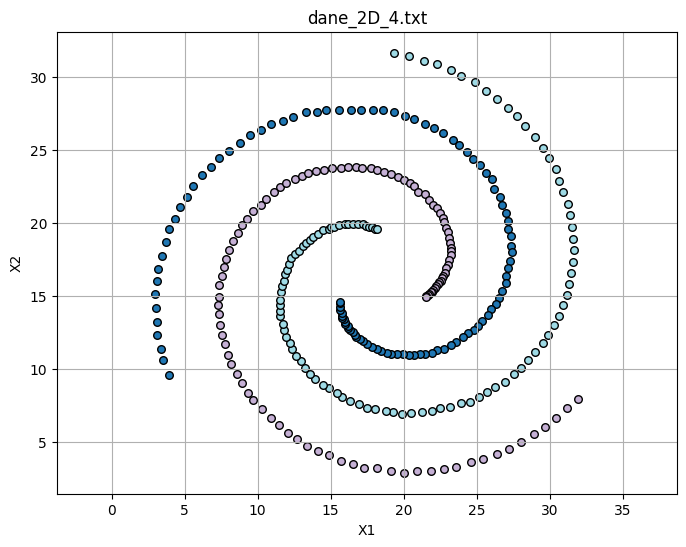
\includegraphics[width=\linewidth]{img/spectral/singular/data4.png}
        \captionsetup{labelformat=empty}
        \caption{Zestaw 4: 3 Klas}
    \end{subfigure}
    \hfill
    \begin{subfigure}[b]{0.30\textwidth}
        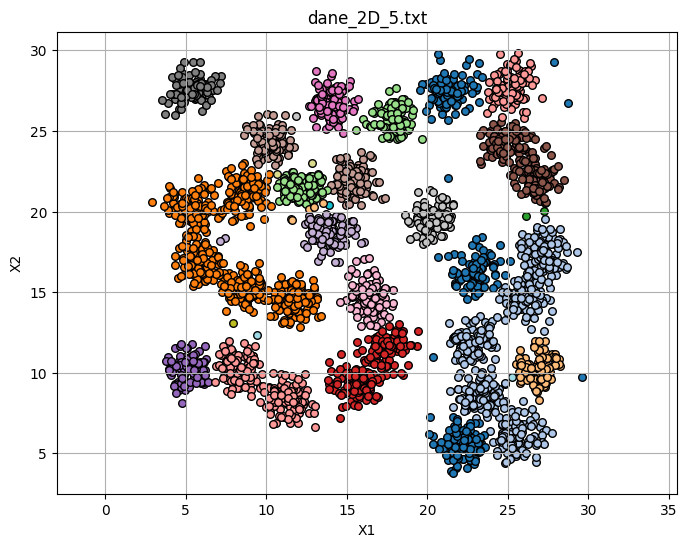
\includegraphics[width=\linewidth]{img/spectral/singular/data5.png}
        \captionsetup{labelformat=empty}
        \caption{Zestaw 5: 31 Klas}
    \end{subfigure}
    \hfill
    \begin{subfigure}[b]{0.30\textwidth}
        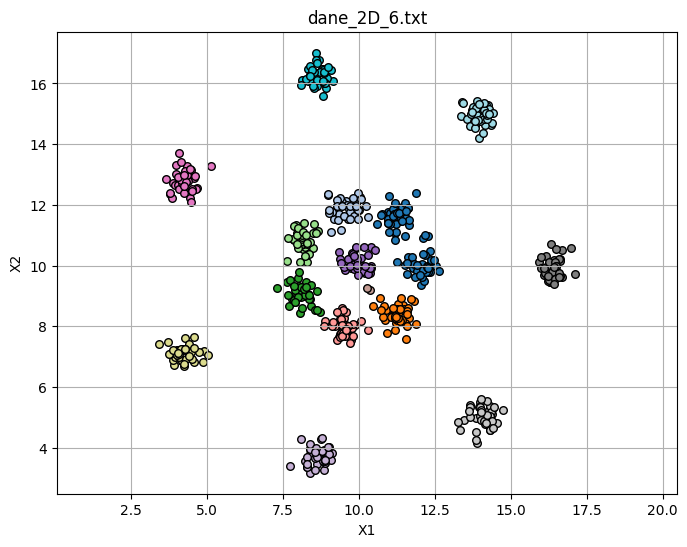
\includegraphics[width=\linewidth]{img/spectral/singular/data6.png}
        \captionsetup{labelformat=empty}
        \caption{Zestaw 6: 15 Klas}
    \end{subfigure}
    \hfill
\end{figure}
\begin{figure}[h!]
    \centering
    \begin{subfigure}[b]{0.30\textwidth}
        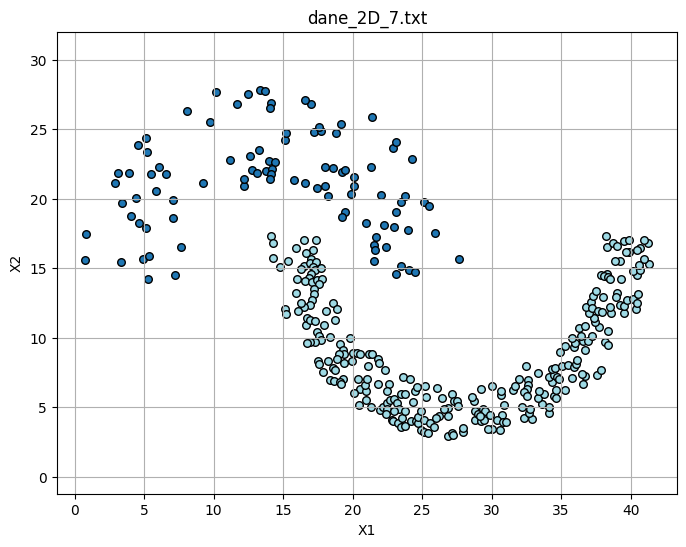
\includegraphics[width=\linewidth]{img/spectral/singular/data7.png}
        \captionsetup{labelformat=empty}
        \caption{Zestaw 7: 2 Klasy}
    \end{subfigure}
    \begin{subfigure}[b]{0.30\textwidth}
        \includegraphics[width=\linewidth]{img/spectral/singular/data8.png}
        \captionsetup{labelformat=empty}
        \caption{Zestaw 8: 2 Klasy}
    \end{subfigure}
    \label{fig:data_grid}
\end{figure} \FloatBarrier



\begin{table}[h!]
\centering
\begin{tabular}{|l|c|}
\hline
\textbf{Zestaw} & \textbf{Dokładność} \\
\hline
Zestaw nr 1 & 0.955 \\
Zestaw nr 2 & 0.981 \\
Zestaw nr 3 & 0.772 \\
Zestaw nr 4 & 1.000 \\
Zestaw nr 5 & 0.960 \\
Zestaw nr 6 & 0.990 \\
Zestaw nr 7 & 1.000 \\
Zestaw nr 8 & 0.541 \\
\hline
\end{tabular}
\caption{Dokładności łączenia centroidalnego}
\end{table}

\noindent Zauważmy, że przy tak dobranych parametrach nasz algorytm bajecznie poradził sobie z zestawami 4, 6 i 7, świetny wynik uzyskał też na zestawach nr 1, 2 i 5. Do poprawnego sklasyfikowania zostają zestawy 3 i 8. Zmieniając metodę łączenia klastrów na łączenie centroidalne udało mi się uzyskać następujące wyniki. Jest to najlepszy wynik jaki uzyskałem na tych zbiorach danych.

\begin{figure}[h!]
    \centering
    \begin{subfigure}[b]{0.30\textwidth}
        \includegraphics[width=\linewidth]{img/spectral/mean/data3.png}
        \captionsetup{labelformat=empty}
        \caption{$\sigma = 1$, dokładność 0.853}
    \end{subfigure}
    \hspace{}
    \begin{subfigure}[b]{0.30\textwidth}
        \includegraphics[width=\linewidth]{img/spectral/mean/data8.png}
        \captionsetup{labelformat=empty}
        \caption{$\sigma = 0.25$, dokładność 0.967}
    \end{subfigure}

    \label{fig:data_grid}
\end{figure} \FloatBarrier

\section{Dane 18D i metoda sylwetkowa}
Zacznijmy od analizy z użyciem metody łokciowej. Wykresy zależności błędu od liczby klastrów przedstawiają się następująco.

\begin{figure}[h!]
    \centering
    \begin{subfigure}[b]{0.30\textwidth}
        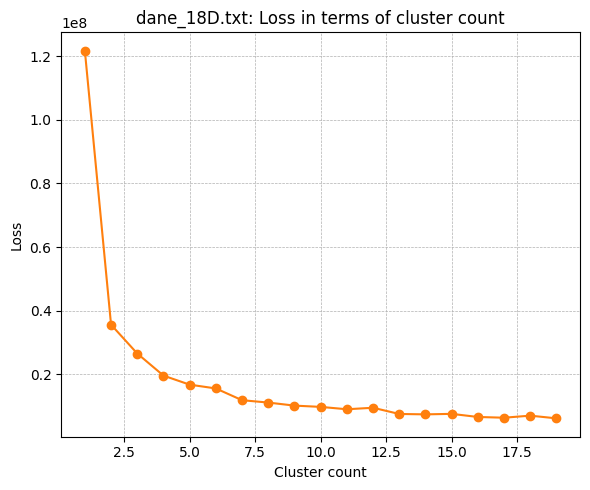
\includegraphics[width=\linewidth]{img/elbow/data18d_manhattan.png}
        \captionsetup{labelformat=empty}
        \caption{Metryka Manhattan}
    \end{subfigure}
    \hspace{}
    \begin{subfigure}[b]{0.30\textwidth}
        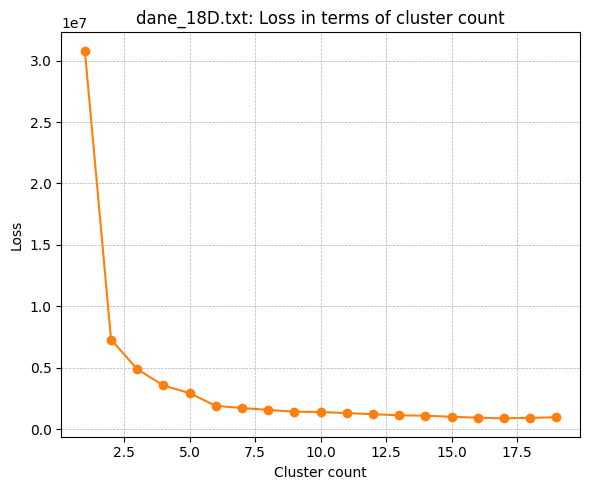
\includegraphics[width=\linewidth]{img/elbow/data18d.png}
        \captionsetup{labelformat=empty}
        \caption{Metryka Euklidesowa}
    \end{subfigure}

    \label{fig:data_grid}
\end{figure} \FloatBarrier

\noindent Pierwsze co wywnioskowałem, to że w obydwu przypadkach $k = 6$ jest pewnym punktem przełamania. Jednak postanowiłem posłużyć się również metodą sylwetkową w celu ustalenia optymalnego $k$. Jednak w związku z dużym rozmiarem danych spróbowałem uprościć trochę wektor cech. Przyjrzyjmy się macierzy korelacji naszych danych
\begin{figure}[h!]
\centering
        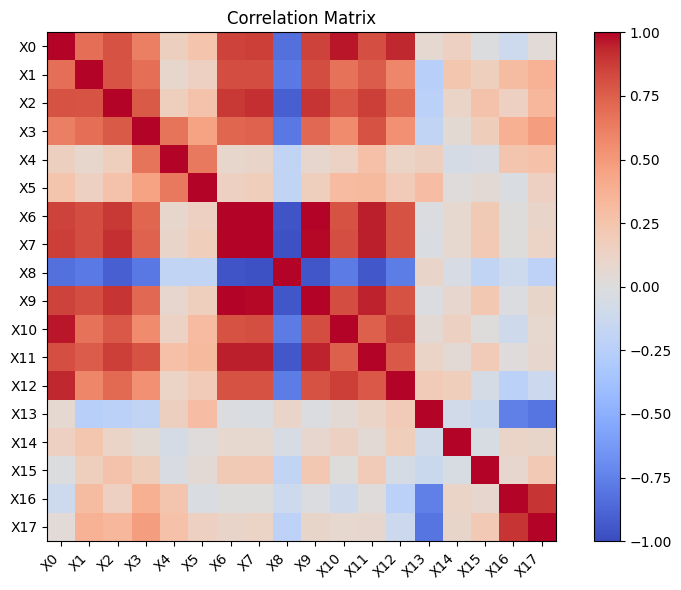
\includegraphics[width=0.4\linewidth]{img/corr.png}
        \captionsetup{labelformat=empty}
        \caption{Macierz korelacji}
\end{figure} \FloatBarrier
Widzimy że wiele cech jest między sobą silnie zależnych, więc spośród nich wszystkich wybrałem cechy $[0, 4, 5, 6, 13, 14, 15, 16, 17]$. Jednak zdziwił mnie wynik metody sylwetkowej więc algorytm powtórzyłem na zbiorze danych bez zależności.

\begin{figure}[h!]
    \centering
    \begin{subfigure}[b]{0.30\textwidth}
        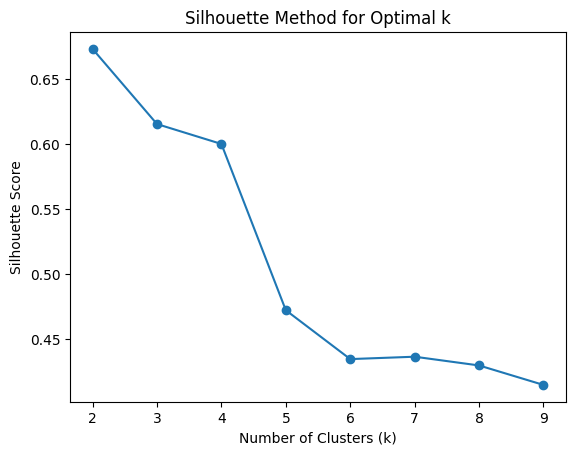
\includegraphics[width=\linewidth]{img/silhouette_full.png}
        \captionsetup{labelformat=empty}
        \centering
        \caption{Metoda sylwestkowa dla pełnego zbioru}
    \end{subfigure}
    \hspace{}
    \begin{subfigure}[b]{0.30\textwidth}
        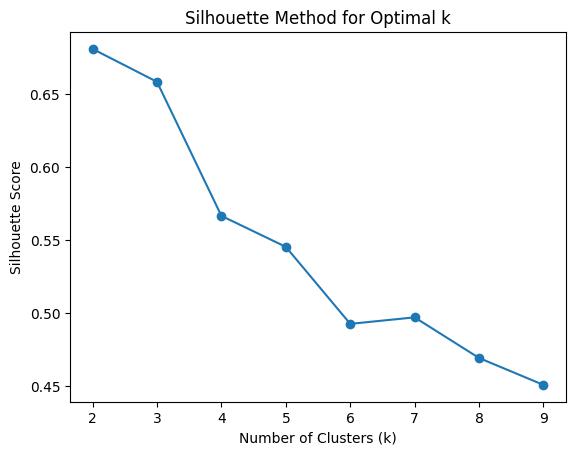
\includegraphics[width=\linewidth]{img/sillhouette_reduced.png}
        \captionsetup{labelformat=empty}
        \centering
        \caption{Metoda sylwetkowa dla uproszczonego zbioru}
    \end{subfigure}

    \label{fig:data_grid}
\end{figure} \FloatBarrier

\noindent Widzimy że w obydwu przypadkach szczyt wykresu przypada dla $k = 2$. Mimo że wnioski dla obu metod się nie pokrywają, to optymalna liczba klas jest gdzieś pomiędzy $2$ i $6$. \smallskip \\
Korzystając z okazji, sprawdźmy jak metoda sylwetkowa poradzi sobie na wyznaczaniu liczby cech dla zestawów 3, 4, 5 i 6. Ze względu na kształt danych, dla zestawu $4$ używam łączenia pojedynczego, a dla pozostałych łączenia centroidalnego. Spójrzmy na wykresy dla naszych danych


\begin{figure}[h!]
    \centering
    \begin{subfigure}[b]{0.30\textwidth}
        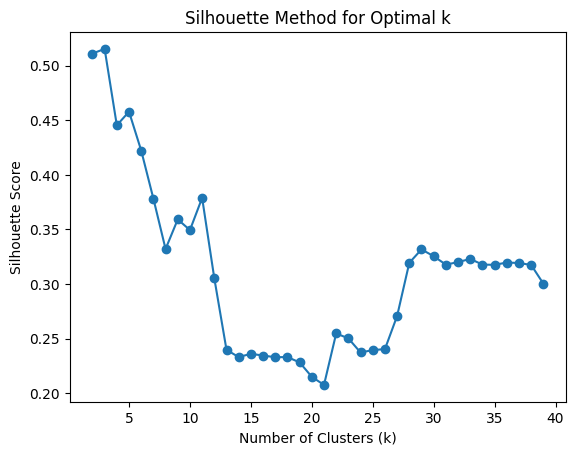
\includegraphics[width=\linewidth]{img/silhouette3.png}
        \captionsetup{labelformat=empty}
        \centering\caption{Metoda sylwestkowa dla zestawu 3}
    \end{subfigure}
    \hspace{}
    \begin{subfigure}[b]{0.30\textwidth}
        \includegraphics[width=\linewidth]{img/silhouette4.png}
        \captionsetup{labelformat=empty}
        \centering
        \centering\caption{Metoda sylwetkowa dla zestawu 4}
    \end{subfigure}
    \hspace{}
    \begin{subfigure}[b]{0.30\textwidth}
        \includegraphics[width=\linewidth]{img/silhouette6.png}
        \captionsetup{labelformat=empty}
        \centering
        \centering\caption{Metoda sylwetkowa dla zestawu 6}
    \end{subfigure}

    \label{fig:data_grid}
\end{figure} \FloatBarrier

\noindent Widzimy, że dla zestawu 3 maximum występuje dla $k = 3$, dla zestawu 4 dla $k = 2$, a dla zestawu 6 dla $k = 16$. Niestety brakuje tu danych dla zestawu $5$, gdyż tą sekcję robiłem bliżej deadline i miałem jeszcze kilka algorytmów do odpalenia, i jak zobaczyłem że po $3h$ jeszcze się nie policzyło to się poddałem. \smallskip \\
W tym przypadku metoda sylwetkowa okazała się być bardzo skuteczna (z dokładnością +/- 1), zatem w ostatecznym rozrachunku skłaniałbym się w kierunku $2$ klas dla danych 18D. Na koniec porównajmy nasze modele na znanym nam z wcześniejszego projektu pliku.


\section{Plik rp.data}
W tym rozdziale chciałbym przedstawić wyniki moich modeli na pliku \texttt{rp.data}, biorąc liczbę klas $k = 2$.

\begin{table}[h!]
\centering
\begin{tabular}{|l|c|}
\hline
\textbf{Model} & \textbf{Accuracy} \\
\hline
KMeans (Euclidean Metric (E)) & 0.924 \\
KMeans (Hamming Metric (H)) & 0.545 \\
KMeans (Manhattan Metric (M)) & 0.897 \\
Hierarchical (E, Singular) & 0.545 \\
Hierarchical (E, Full) & 0.800 \\
Hierarchical (E, Mean) & 0.892 \\
Hierarchical (E, Centroid) & 0.545 \\
Hierarchical (E, Ward) & 0.929 \\
Hierarchical (M, Full) & 0.837 \\
Hierarchical (M, Mean) & 0.887 \\
Hierarchical (M, Ward) & 0.932 \\
Spectral (E, $\sigma = 0.0125$) & 0.897 \\
Spectral (E, $\sigma = 0.05$) & 0.854 \\
Spectral (E, $\sigma = 0.5$) & 0.547 \\
\hline
\end{tabular}
\caption{Benchmark modeli na zbiorze rp.data}
\end{table}

\section{Podsumowanie}
Porównując algorytmy, każdy z nich przydaje się do różnych zbiorów danych. Były przypadki gdy algorytm \texttt{k-średnich} radził sobie najlepiej, w innych \texttt{grupowanie hierarchiczne} czy \texttt{klasteryzacja spektralna} wypadały lepiej. Jednak najszybszy z nich zdecydowanie był algorytm \texttt{k-średnich}. Różne kombinacje różnych ustawień sprawdzały się inaczej dla każdego ze zbiorów danych. Zaskakująco, algorytm \texttt{k-średnich} zdominował przy pliku \texttt{rp.data}, pokonywało go nieznacznie grupowanie hierarchiczne dla metryki Manhattan i Łączenia Warda. Dla klasteryzacji spektralnej było jeszcze więcej parametrów, bo nie tylko kontrolowaliśmy końcowy algorytm łączenia ale również hiperparametr $\sigma$, który zachowywał się różnie dla różnych zbiorów danych. \smallskip \\
Porównując różne metody wyznaczania liczby klastrów, żadna nie wypadła bezkonkurencyjnie. Metoda łokciowa nie była łatwa do rozczytania, za to dosyć szybka bo korzystała z algorytmy k-średnich. Z drugiej strony metoda sylwetkowa często dawała jednoznaczny rezultat, ale z uwagi na wykorzystanie grupowania hierarchicznego była kosztowna obliczeniowo. Bywało też tak że analizując dane obydwoma metodami dochodziłem do różnych wniosków. \smallskip \\
Ostatecznie na wszystkich zbiorach osiągnąłem zadowalający wynik, jednak nie było algorytmu który poradziłby sobie przyzwoicie w każdej sytuacji.
\end{document}
